\documentclass{beamer}

\usepackage{txfonts}
\usepackage{hyperref}
\usepackage{fancybox}
\usepackage{xfrac}
\usepackage{cancel}
\usepackage{slashbox}


\newcommand{\heart}{\ensuremath\heartsuit}

\usepackage{mathtools,amssymb}
\newcommand{\myarrow}{\scalebox{2}[2]{$\mathclap{\curvearrowleft}\mkern2.2mu
                                                 \mathclap{\curvearrowright}$}}

\DeclareMathOperator{\Bin}{\mathrm{Bin}}

\hypersetup{colorlinks=false,linkbordercolor=red,linkcolor=green,pdfborderstyle={/S/U/W 1}}

\addtobeamertemplate{navigation symbols}{}{ \hspace{1em}    \usebeamerfont{footline}%
    \insertframenumber / \inserttotalframenumber}

\geometry{papersize={15cm,13cm}}
\usepackage{lipsum}

\makeatletter
\newenvironment<>{contdproof}[1][\proofname]{%
    \par
    \def\insertproofname{#1\@addpunct{.}}%
    \usebeamertemplate{proof begin}#2}
  {\usebeamertemplate{proof end}}
\makeatother


\setbeamertemplate{theorems}[numbered]

\newtheorem*{nonumdefinition}{Definition}
\newtheorem*{nonumproblem}{Problem}
\newtheorem*{nonumlemma}{Lemma}
\newtheorem*{nonumtheorem}{Theorem}
\newtheorem*{nonumproof}{Proof}
\newtheorem*{nonumremark}{Remark}
\newtheorem*{answer}{Answer}
\newtheorem*{nonumremarks}{Remarks}
\newtheorem*{nonumexamples}{Examples}
\newtheorem*{nonumsolution}{Solution}
\newtheorem*{nonumexample}{Example}
\newtheorem*{nonumproposition}{Proposition}

\newtheorem{remark}{Remark}
\newtheorem{exam}{Example}




\theoremstyle{alphtheorem}
\newtheorem{alphtheorem}{Theorem}
\renewcommand{\thealphtheorem}{\Alph{alphtheorem}}
\renewcommand{\thesection}{\arabic{section}}



\usepackage{tikz}
\newcommand*\mycirc[1]{%
  \tikz[baseline=(C.base)]\node[draw,circle,inner sep=.7pt](C) {#1};\:
}

\newcommand\myheading[1]{%
  \par\bigskip
  {\color{blue}{\large #1}}\par\smallskip}

%\usetheme{Warsaw}
%\usetheme{Berkeley} %sample 1

\usetheme{Berlin} % sample 2
%\usetheme{AnnArbor} % sample 3

\let\otp\titlepage
\renewcommand{\titlepage}{\otp\addtocounter{framenumber}{-1}}

\title{Lecture 19: More Than Two Random Variables}
\author{}
\date{}

\begin{document}
\begin{frame}[plain]
\titlepage
\end{frame}

\begin{frame}
\begin{nonumdefinition}
If $X_1, X_2, \ldots, X_n$ are discrete random variables defined on the same sample space then their joint pmf is the function
$$
P_{X_1, X_2, \ldots, X_n} (x_1, x_2, \ldots, x_n) = P(X_1 = x_1, \ldots, X_n = x_n)
$$
If $X_1, X_2, \ldots, X_n$ are continuous then their joint pdf is the function $f_{X_1, X_2, \ldots, X_n} (x_1, x_2, \ldots, x_n)$ such that 
\end{nonumdefinition}
\end{frame}

\begin{frame}
\begin{nonumdefinition}[Cont.]
for any region $A$ in $\mathbb{R}^n$
$$
P((X_1, X_2, \ldots, X_n) \in A) = \underbrace{\int\limits \ldots \int\limits_A f_{X_1, X_2, \ldots, X_n} (x_1, \ldots, x_n) dx_1, \ldots, dx_n}_{\text{$n$-fold multiple integral}}
$$
\end{nonumdefinition}

\begin{nonumdefinition}
The discrete random variables $X_1, X_2, \ldots, X_n$ are independent if 
$$
P_{X_1, \ldots, X_n} (x_1, \ldots, x_n) = P_{X_1} (x_1) P_{X_2} (x_2) \ldots P_{X_n} (x_n).
$$
Equivalently
$$
P(X_1 = x_1, \ldots, X_n = x_n) = P(X_1 = x_1) \ldots  P(X_n = x_n)
$$
\end{nonumdefinition}
\end{frame}

\begin{frame}
The continuous random variables $X_1, X_2, \ldots, X_n$ are independent if 
$$
f_{X_1, X_2,\ldots, X_n} (x_1, x_2, \ldots, x_n) = f_{X_1}  (x_1) f_{X_2} (x_2) \ldots f_{X_n} (x_n)
$$

\begin{nonumdefinition}
$X_1, X_2, \ldots, X_n$ are {\it pairwise independent} if each pair $X_i, X_j (i \neq j)$ is independent.  We will now see
\begin{tabbing}
Pairwise independence \= $\not{\Longrightarrow}$ \= Independence\\
of random variables  \> $\Longleftarrow$ \> of random variables\\
\end{tabbing}
\end{nonumdefinition}
\end{frame}

\begin{frame}
First we will prove $\Longleftarrow$

\begin{nonumtheorem}
$X_1, X_2, \ldots, X_n$ independent  $\Rightarrow$ $X_1, X_2, \ldots, X_n$ are pairwise independent.
\end{nonumtheorem}

From now on we will restrict to the case $n=3$ so we have THREE random variables $X,Y,Z$.
\end{frame}

\begin{frame}
How do we get
$$
P_{X,Y} (x, y) \text{~~ from ~~} P_{X,Y,Z} (x,y,z)
$$

Answer (left to you to prove)
\begin{align*}
P_{X,Y} (x,y) = \sum\limits_{\text{all } z} P_{X,Y,Z} (x,y,z) \tag{$\#$}
\end{align*}

Now we can prove $X,Y,Z$ independent.
$$
\Longrightarrow ~~ X,Y \text{ independent}
$$
\end{frame}

\begin{frame}
Since $X,Y,Z$ are independent we have 
\begin{equation*}
P_{X,Y,Z} (x,y,z) = P_X(x) P_Y (y) P_Z (z) \tag{$\#\#$}
\end{equation*}

Now play the RHS of ($\#\#$) into the RHS of ($\#$)

\medskip
\centerline{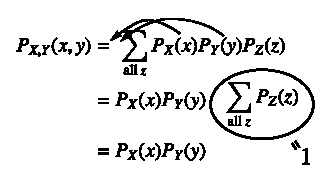
\includegraphics{figure/art19(1).eps}}
\end{frame}

\begin{frame}
This proves $X$ and $Y$ are independent Identical proofs prove the pairs $X$, $Z$ and $Y$, $Z$ are independent.

Now we construct $X,Y,Z$ (actually $X_A$, $X_B$, $X_C$) so that each {\it pair} is  independent but the triple $X,Y,Z$ is {\it not} {\it independent}.
\end{frame}

\begin{frame}
\myheading{A Variation on the Cool Counter example}

Lets go back to the ``cool counter example'', Lecture 16, page 18 of three events $A,B,C$ which are pairwise independent but no independent so
$$
P(A \cap B \cap C) \neq P(A) P(B) P(C)
$$
The idea is to convert the three events to random variables $X_A, X_B, X_C$ so that 

$X_A = 1$ on $A$ and $O$ on $A$' etc.
\end{frame}

\begin{frame}
In fact we won't need the corner points $(-1, -1)$, $(-1,1)$, $(1,-1)$  and $(1,1)$ we put $S_1 =(0,1)$, $S_2= (-1,0)$, $S_3 = (0,1)$, $S_4 = (1,0)$ and retain their probabilities so
$$
P(\{S_j\}) = \frac{1}{4}, \quad 1 \leq j \leq 4
$$
\medskip
\centerline{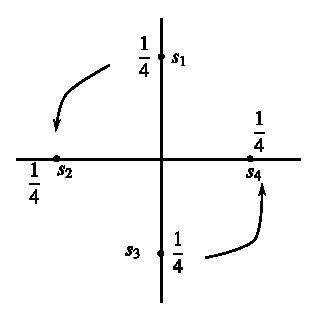
\includegraphics{figure/art19(2).eps}}
\end{frame}

\begin{frame}
We define 
\begin{align*}
A & = \{s_1, s_2\}\\
B & = \{s_1 , s_3\}\\
C & = \{s_1 , s_4\}
\end{align*}

\medskip
\centerline{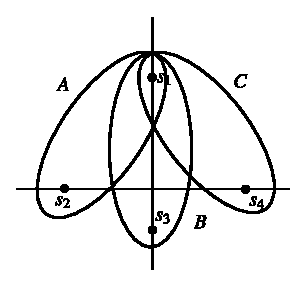
\includegraphics{figure/art19(3).eps}}


We define $X_A$, $X_B$, $X_C$ on $S$ by 
$$
X_A (s_j) = 
\begin{cases}
1, ~~ \text{ if } s_j \in A\\
0, ~~ \text{ if } s_j \not\in A
\end{cases}
$$
\end{frame}

\begin{frame}
$$
X_B (s_j)  = 
\begin{cases}
1, ~~ \text{ if } s_j \in B\\
0, ~~ \text{ if } s_j \not\in B
\end{cases}
$$
$$
X_C (s_j) = 
\begin{cases}
1, \text{ if } s_j \in C\\
0, \text{ if } s_j \not\in C
\end{cases}
$$
\begin{align*}
\text{So } \quad & P(X_A = 1) = P(\{S_1, S_2\}) = \frac{1}{2}\\
& P(X_A = 0) = P(\{S_3, S_4\}) = \frac{1}{2}
\end{align*}
and similarly for $X_B$ and $X_C$.
$$
\text{ So } \qquad X_A, X_B \text{~ and ~} X_C
$$
are Bernoulli random variables 
\end{frame}

\begin{frame}
Let's compute the joint pmf of $X_A$ and $X_B$. We know the margin

\begin{center}
\begin{tabular}{c|c|c|c}
\backslashbox{$X_A$}{$X_B$} & 0 & 1 & \\
\hline
0 &  & & $\sfrac{1}{2}$\\
\hline
1 &  &  & $\sfrac{1}{2}$\\
\hline
& $\sfrac{1}{2}$ & $\sfrac{1}{2}$ &
\end{tabular}
\end{center}

The subset where $X_A  =1$ is the subset $\{s_1, s_2\}$ so we write an equality of events
$$
(X_A =1) = \{s_1, s_2\}
$$
Similarly
\begin{gather*}
(X_A =0) = \{s_3 , s_4\}\\
(X_B =1)  = \{s_1 , x_3\}, (X_B =0) = \{s_2 , s_4\}\\
(X_C =1) = \{s_1, s_4\}, (X_C =0) = \{s_2, s_3\}
\end{gather*}
\end{frame}

\begin{frame}
Hence 
\begin{align*}
(X_A = 0) \cap (X_B =0) & = \{S_4\}\\
\text{so } \qquad P(X_A = 0, X_B = 0) & = \dfrac{1}{4}\\
(X_A = 0) \cap (X_B = 1) & = \{S_3\}\\
\text{so } \qquad P(X_A = 0, X_B = 1) & = \dfrac{1}{4}\\
(X_A = 1) \cap (X_B =0) & = \{S_2\}\\
P(X_A =1, X_B =0) & = \frac{1}{4}\\
(X_A =1) \cap (X_B =1) & = \{S_1\}\\
P(X_A =1, X_B =1) & = P(\{S_1\}) = \frac{1}{4}
\end{align*} 
etc.
\end{frame}

\begin{frame}
So the joint proof of $X_A$ and $X_B$ is 
\begin{center}
\begin{tabular}{c|c|c|c}
\backslashbox{$X_A$}{$X_B$} & 0 & 1 & \\
\hline
0 & $\sfrac{1}{4}$ & $\sfrac{1}{4}$ & $\sfrac{1}{2}$\\
\hline
1 & $\sfrac{1}{4}$ & $\sfrac{1}{4}$ & $\sfrac{1}{2}$\\
\hline
& $\sfrac{1}{2}$ & $\sfrac{1}{2}$ &
\end{tabular}
\end{center}
so $X_A$ and $X_B$ are independent.  The same is true for $X_A$ and $X_C$ and $X_B$ and $\chi_C$.

Now we show the triple $X_A$, $X_B$ and $X_C$ is NOT independent.
\end{frame}

\begin{frame}
We will show 
\begin{multline*}
\hspace{2.5cm} P(X_A = 1, X_B = 1, X_C = 1)\\
\neq P(X_A =1) P(X_B = 1) P(X_C = 1) \hspace{2.5cm} 
\end{multline*}

The RHS $= \left(\dfrac{1}{2} \right) \left(\dfrac{1}{2} \right) \left(\dfrac{1}{2} \right) = \dfrac{1}{8}$

The left-hand side is the probability of the event 
\begin{align*}
&(X_A =1) \cap (X_B = 1) \cap (X_C =1)\\
& = \{S_1, S_2\} \cap \{S_1, S_3\} \cap \{S_1, S_4\}\\
& = \{S_1\}.
\end{align*}
\end{frame}

\begin{frame}
So
$$
P(X_A =1, X_B =1, X_C =1) = P(\{S_1\}) = \frac{1}{4}
$$
so 
\begin{align*}
\text{LHS} & = \frac{1}{4}\\
\text{RHS} & = \frac{1}{8}
\end{align*}

\begin{nonumremark}
This counter example is more or less the some as the ``cool counter example''. We just replaced (more or less) $A, B, C$ by their ``characteristic functions''.
\end{nonumremark}
\end{frame}

\end{document}




